\documentclass[12pt]{article}
\usepackage{latexblog}

% ============================================================
% Blog Metadata
% ============================================================
\blogtitle{理解Java并发(5)：AQS}
\blogdate{2020-06-01}
\blogtags{AQS, 并发编程, Concurrent, ~理解Java并发, 刨根问底}
\bloglang{zh}
\blogsummary{}

\begin{document}
\makeblogtitle

AQS(AbstractQueuedSynchronizer)是一个机遇FIFO等待队列实现锁的框架，用来实现诸如ReentrantLock、Semaphore等。

\begin{Shaded}
\begin{Highlighting}[]
\KeywordTok{public} \KeywordTok{abstract} \KeywordTok{class} \BuiltInTok{AbstractQueuedSynchronizer}
\KeywordTok{extends} \BuiltInTok{AbstractOwnableSynchronizer}
\KeywordTok{implements} \BuiltInTok{Serializable}
\end{Highlighting}
\end{Shaded}

\section{基本用法}\label{ux57faux672cux7528ux6cd5}

AQS在类里面维护了一个原子int类型的状态值（这个值的具体含义由子类去定义）。要使用AQS，推荐的做法是在在一个私有的内部类中去实现AQS，然后需要通过AQS本身提供的几个方法：

\begin{itemize}
\tightlist
\item
  \texttt{getState()}
\item
  \texttt{setState(int)}
\item
  \texttt{compareAndSetState(int,\ int)}
\end{itemize}

通过调用上述三个方法来维护同步状态，并实现这些方法：

\begin{itemize}
\tightlist
\item
  \texttt{tryAcquire(int)}：尝试获取状态
\item
  \texttt{tryRelease(int)}：尝试释放状态
\item
  \texttt{tryAcquireShared(int)}
\item
  \texttt{tryReleaseShared(int)}
\item
  \texttt{isHeldExclusively()}: 判断当前线程是否持有排它锁
\end{itemize}

而其他的同步操作、队列管理等，在AQS中已经完成了。

\subsection{样例：实现简单的锁}\label{ux6837ux4f8bux5b9eux73b0ux7b80ux5355ux7684ux9501}

在AQS的文档中给了一个基本的用法:实现一个不可重入的锁。首先需要的就是实现内部的类：

\begin{Shaded}
\begin{Highlighting}[]
\KeywordTok{class}\NormalTok{ Mutex }\KeywordTok{implements} \BuiltInTok{Lock}\OperatorTok{,}\NormalTok{ java}\OperatorTok{.}\FunctionTok{io}\OperatorTok{.}\FunctionTok{Serializable} \OperatorTok{\{}
   \KeywordTok{private} \DataTypeTok{static} \KeywordTok{class}\NormalTok{ Sync }\KeywordTok{extends} \BuiltInTok{AbstractQueuedSynchronizer} \OperatorTok{\{}
     \KeywordTok{protected} \DataTypeTok{boolean} \FunctionTok{isHeldExclusively}\OperatorTok{()} \OperatorTok{\{}
       \ControlFlowTok{return} \FunctionTok{getState}\OperatorTok{()} \OperatorTok{==} \DecValTok{1}\OperatorTok{;}
     \OperatorTok{\}}

     \KeywordTok{public} \DataTypeTok{boolean} \FunctionTok{tryAcquire}\OperatorTok{(}\DataTypeTok{int}\NormalTok{ acquires}\OperatorTok{)} \OperatorTok{\{}
       \ControlFlowTok{assert}\NormalTok{ acquires }\OperatorTok{==} \DecValTok{1}\OperatorTok{;} \CommentTok{// Otherwise unused}
       \ControlFlowTok{if} \OperatorTok{(}\FunctionTok{compareAndSetState}\OperatorTok{(}\DecValTok{0}\OperatorTok{,} \DecValTok{1}\OperatorTok{))} \OperatorTok{\{}
         \FunctionTok{setExclusiveOwnerThread}\OperatorTok{(}\BuiltInTok{Thread}\OperatorTok{.}\FunctionTok{currentThread}\OperatorTok{());}
         \ControlFlowTok{return} \KeywordTok{true}\OperatorTok{;}
       \OperatorTok{\}}
       \ControlFlowTok{return} \KeywordTok{false}\OperatorTok{;}
     \OperatorTok{\}}

     \KeywordTok{protected} \DataTypeTok{boolean} \FunctionTok{tryRelease}\OperatorTok{(}\DataTypeTok{int}\NormalTok{ releases}\OperatorTok{)} \OperatorTok{\{}
       \ControlFlowTok{assert}\NormalTok{ releases }\OperatorTok{==} \DecValTok{1}\OperatorTok{;} \CommentTok{// Otherwise unused}
       \ControlFlowTok{if} \OperatorTok{(}\FunctionTok{getState}\OperatorTok{()} \OperatorTok{==} \DecValTok{0}\OperatorTok{)} \ControlFlowTok{throw} \KeywordTok{new} \BuiltInTok{IllegalMonitorStateException}\OperatorTok{();}
       \FunctionTok{setExclusiveOwnerThread}\OperatorTok{(}\KeywordTok{null}\OperatorTok{);}
       \FunctionTok{setState}\OperatorTok{(}\DecValTok{0}\OperatorTok{);}
       \ControlFlowTok{return} \KeywordTok{true}\OperatorTok{;}
     \OperatorTok{\}}
   \OperatorTok{\}}
   \CommentTok{// ...}
\OperatorTok{\}}
\end{Highlighting}
\end{Shaded}

然后，加锁、解锁等操作都可以通过这个内部类来完成了：

\begin{Shaded}
\begin{Highlighting}[]
\KeywordTok{class}\NormalTok{ Mutex }\KeywordTok{implements} \BuiltInTok{Lock}\OperatorTok{,}\NormalTok{ java}\OperatorTok{.}\FunctionTok{io}\OperatorTok{.}\FunctionTok{Serializable} \OperatorTok{\{}
   \CommentTok{// ...}
   \KeywordTok{private} \DataTypeTok{final}\NormalTok{ Sync sync }\OperatorTok{=} \KeywordTok{new} \FunctionTok{Sync}\OperatorTok{();}

   \CommentTok{// 这里通过获取或者释放状态1（1表示锁定）来实现加锁和解锁的操作}
   \KeywordTok{public} \DataTypeTok{void} \FunctionTok{lock}\OperatorTok{()}                \OperatorTok{\{}\NormalTok{ sync}\OperatorTok{.}\FunctionTok{acquire}\OperatorTok{(}\DecValTok{1}\OperatorTok{);} \OperatorTok{\}}
   \KeywordTok{public} \DataTypeTok{boolean} \FunctionTok{tryLock}\OperatorTok{()}          \OperatorTok{\{} \ControlFlowTok{return}\NormalTok{ sync}\OperatorTok{.}\FunctionTok{tryAcquire}\OperatorTok{(}\DecValTok{1}\OperatorTok{);} \OperatorTok{\}}
   \KeywordTok{public} \DataTypeTok{void} \FunctionTok{unlock}\OperatorTok{()}              \OperatorTok{\{}\NormalTok{ sync}\OperatorTok{.}\FunctionTok{release}\OperatorTok{(}\DecValTok{1}\OperatorTok{);} \OperatorTok{\}}
   \KeywordTok{public} \BuiltInTok{Condition} \FunctionTok{newCondition}\OperatorTok{()}   \OperatorTok{\{} \ControlFlowTok{return}\NormalTok{ sync}\OperatorTok{.}\FunctionTok{newCondition}\OperatorTok{();} \OperatorTok{\}}
   \KeywordTok{public} \DataTypeTok{boolean} \FunctionTok{isLocked}\OperatorTok{()}         \OperatorTok{\{} \ControlFlowTok{return}\NormalTok{ sync}\OperatorTok{.}\FunctionTok{isHeldExclusively}\OperatorTok{();} \OperatorTok{\}}
   \KeywordTok{public} \DataTypeTok{boolean} \FunctionTok{hasQueuedThreads}\OperatorTok{()} \OperatorTok{\{} \ControlFlowTok{return}\NormalTok{ sync}\OperatorTok{.}\FunctionTok{hasQueuedThreads}\OperatorTok{();} \OperatorTok{\}}
   \KeywordTok{public} \DataTypeTok{void} \FunctionTok{lockInterruptibly}\OperatorTok{()} \KeywordTok{throws} \BuiltInTok{InterruptedException} \OperatorTok{\{}
\NormalTok{     sync}\OperatorTok{.}\FunctionTok{acquireInterruptibly}\OperatorTok{(}\DecValTok{1}\OperatorTok{);}
   \OperatorTok{\}}
   \KeywordTok{public} \DataTypeTok{boolean} \FunctionTok{tryLock}\OperatorTok{(}\DataTypeTok{long}\NormalTok{ timeout}\OperatorTok{,} \BuiltInTok{TimeUnit}\NormalTok{ unit}\OperatorTok{)} \KeywordTok{throws} \BuiltInTok{InterruptedException} \OperatorTok{\{}
     \ControlFlowTok{return}\NormalTok{ sync}\OperatorTok{.}\FunctionTok{tryAcquireNanos}\OperatorTok{(}\DecValTok{1}\OperatorTok{,}\NormalTok{ unit}\OperatorTok{.}\FunctionTok{toNanos}\OperatorTok{(}\NormalTok{timeout}\OperatorTok{));}
   \OperatorTok{\}}
 \OperatorTok{\}}
\end{Highlighting}
\end{Shaded}

\section{原理}\label{ux539fux7406}

AQS内部是使用的基于CLH队列的同步机制。

\begin{figure}
\centering
\pandocbounded{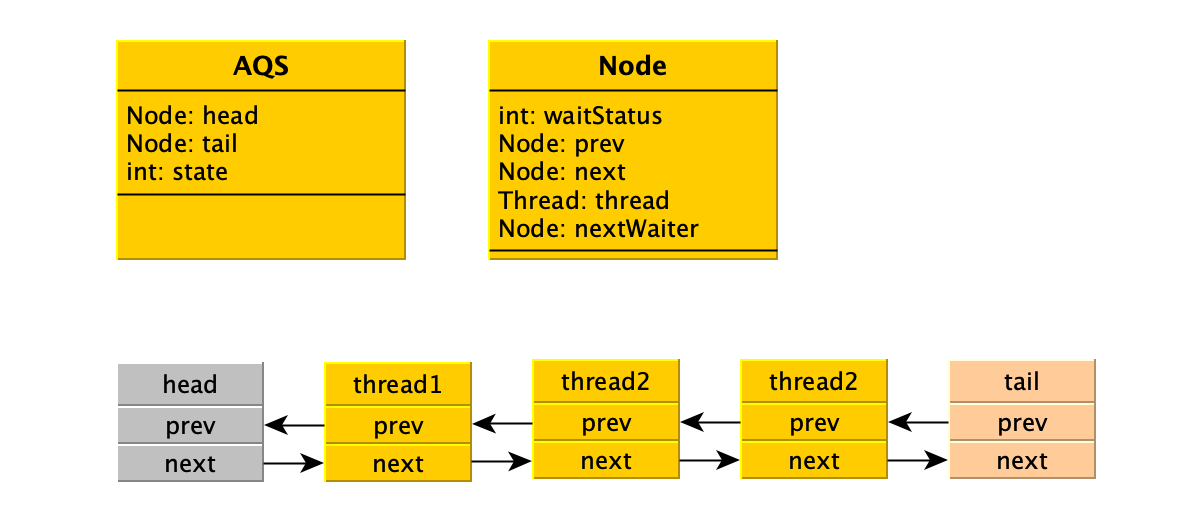
\includegraphics[keepaspectratio,alt={AQS CLH}]{images/AQS_queue.png}}
\caption{AQS CLH}
\end{figure}

\subsection{acquire获取状态}\label{acquireux83b7ux53d6ux72b6ux6001}

acquire意味着尝试通过获取某个状态从而获取到锁。acquire的过程如下：

\begin{itemize}
\tightlist
\item
  首先尝试直接通过CAS的方式改变state，如果成功则直接获取到锁
\item
  如果上一步失败，那么表明其他线程获取到锁，则尝试将当前线程加入到队列末尾进行排队（同样加入到队列末尾也是通过CAS实现）
\item
  加入到队列后，中断当前线程（但具体线程如何处理中断要看线程自己了）
\end{itemize}

\begin{Shaded}
\begin{Highlighting}[]
\KeywordTok{public} \DataTypeTok{final} \DataTypeTok{void} \FunctionTok{acquire}\OperatorTok{(}\DataTypeTok{int}\NormalTok{ arg}\OperatorTok{)} \OperatorTok{\{}
    \ControlFlowTok{if} \OperatorTok{(!}\FunctionTok{tryAcquire}\OperatorTok{(}\NormalTok{arg}\OperatorTok{)} \OperatorTok{\&\&} \FunctionTok{acquireQueued}\OperatorTok{(}\FunctionTok{addWaiter}\OperatorTok{(}\BuiltInTok{Node}\OperatorTok{.}\FunctionTok{EXCLUSIVE}\OperatorTok{),}\NormalTok{ arg}\OperatorTok{))}
        \FunctionTok{selfInterrupt}\OperatorTok{();}
\OperatorTok{\}}
\end{Highlighting}
\end{Shaded}

\begin{Shaded}
\begin{Highlighting}[]
\KeywordTok{private} \BuiltInTok{Node} \FunctionTok{addWaiter}\OperatorTok{(}\BuiltInTok{Node}\NormalTok{ mode}\OperatorTok{)} \OperatorTok{\{}
    \BuiltInTok{Node}\NormalTok{ node }\OperatorTok{=} \KeywordTok{new} \BuiltInTok{Node}\OperatorTok{(}\BuiltInTok{Thread}\OperatorTok{.}\FunctionTok{currentThread}\OperatorTok{(),}\NormalTok{ mode}\OperatorTok{);}
    \BuiltInTok{Node}\NormalTok{ pred }\OperatorTok{=}\NormalTok{ tail}\OperatorTok{;}
    \CommentTok{// 如果发现队列不为空，那么尝试一次性快速插入到尾部（如果失败的话则通过enq方法插入）}
    \CommentTok{// 在没有线程竞争的情况下，会比enq稍微快一点，enq里面还要处理队列为空的情况}
    \ControlFlowTok{if} \OperatorTok{(}\NormalTok{pred }\OperatorTok{!=} \KeywordTok{null}\OperatorTok{)} \OperatorTok{\{}
\NormalTok{        node}\OperatorTok{.}\FunctionTok{prev} \OperatorTok{=}\NormalTok{ pred}\OperatorTok{;}
        \ControlFlowTok{if} \OperatorTok{(}\FunctionTok{compareAndSetTail}\OperatorTok{(}\NormalTok{pred}\OperatorTok{,}\NormalTok{ node}\OperatorTok{))} \OperatorTok{\{}
            \CommentTok{// 通过CAS设置tail成功，这时候tail已经是当前node，再把之前的tail（pred）连接到自己}
\NormalTok{            pred}\OperatorTok{.}\FunctionTok{next} \OperatorTok{=}\NormalTok{ node}\OperatorTok{;}
            \ControlFlowTok{return}\NormalTok{ node}\OperatorTok{;}
        \OperatorTok{\}}
    \OperatorTok{\}}
    \CommentTok{// enq的逻辑基本上与上面一样，区别在于1. 处理队列为空的情况，要插入到队列头部；2.CAS失败后会重试直到成功}
    \FunctionTok{enq}\OperatorTok{(}\NormalTok{node}\OperatorTok{);}
    \ControlFlowTok{return}\NormalTok{ node}\OperatorTok{;}
\OperatorTok{\}}
\end{Highlighting}
\end{Shaded}

\begin{Shaded}
\begin{Highlighting}[]
\KeywordTok{private} \BuiltInTok{Node} \FunctionTok{enq}\OperatorTok{(}\DataTypeTok{final} \BuiltInTok{Node}\NormalTok{ node}\OperatorTok{)} \OperatorTok{\{}
    \ControlFlowTok{for} \OperatorTok{(;;)} \OperatorTok{\{}
        \BuiltInTok{Node}\NormalTok{ t }\OperatorTok{=}\NormalTok{ tail}\OperatorTok{;}
        \ControlFlowTok{if} \OperatorTok{(}\NormalTok{t }\OperatorTok{==} \KeywordTok{null}\OperatorTok{)} \OperatorTok{\{}
            \CommentTok{// 如果发现队列为空那么首先把head和tail都设置为空节点}
            \ControlFlowTok{if} \OperatorTok{(}\FunctionTok{compareAndSetHead}\OperatorTok{(}\KeywordTok{new} \BuiltInTok{Node}\OperatorTok{()))}
\NormalTok{                tail }\OperatorTok{=}\NormalTok{ head}\OperatorTok{;}
        \OperatorTok{\}} \ControlFlowTok{else} \OperatorTok{\{}
\NormalTok{            node}\OperatorTok{.}\FunctionTok{prev} \OperatorTok{=}\NormalTok{ t}\OperatorTok{;}
            \ControlFlowTok{if} \OperatorTok{(}\FunctionTok{compareAndSetTail}\OperatorTok{(}\NormalTok{t}\OperatorTok{,}\NormalTok{ node}\OperatorTok{))} \OperatorTok{\{}
\NormalTok{                t}\OperatorTok{.}\FunctionTok{next} \OperatorTok{=}\NormalTok{ node}\OperatorTok{;}
                \ControlFlowTok{return}\NormalTok{ t}\OperatorTok{;}
            \OperatorTok{\}}
        \OperatorTok{\}}
    \OperatorTok{\}}
\OperatorTok{\}}
\end{Highlighting}
\end{Shaded}

\subsection{release操作}\label{releaseux64cdux4f5c}

当释放锁的时候，会唤醒一个后继节点，这个节点通常是后一个节点（如果后一个节点cancel了则要从队列尾部遍历直到找到真正的后继节点）。

\begin{Shaded}
\begin{Highlighting}[]
\KeywordTok{public} \DataTypeTok{final} \DataTypeTok{boolean} \FunctionTok{release}\OperatorTok{(}\DataTypeTok{int}\NormalTok{ arg}\OperatorTok{)} \OperatorTok{\{}
    \ControlFlowTok{if} \OperatorTok{(}\FunctionTok{tryRelease}\OperatorTok{(}\NormalTok{arg}\OperatorTok{))} \OperatorTok{\{}
        \BuiltInTok{Node}\NormalTok{ h }\OperatorTok{=}\NormalTok{ head}\OperatorTok{;}
        \ControlFlowTok{if} \OperatorTok{(}\NormalTok{h }\OperatorTok{!=} \KeywordTok{null} \OperatorTok{\&\&}\NormalTok{ h}\OperatorTok{.}\FunctionTok{waitStatus} \OperatorTok{!=} \DecValTok{0}\OperatorTok{)}
            \FunctionTok{unparkSuccessor}\OperatorTok{(}\NormalTok{h}\OperatorTok{);}
        \ControlFlowTok{return} \KeywordTok{true}\OperatorTok{;}
    \OperatorTok{\}}
    \ControlFlowTok{return} \KeywordTok{false}\OperatorTok{;}
\OperatorTok{\}}
\end{Highlighting}
\end{Shaded}

\begin{itemize}
\tightlist
\item
  \href{http://gee.cs.oswego.edu/dl/papers/aqs.pdf}{The java.util.concurrent Synchronizer Framework}
\end{itemize}


\end{document}
